\section{1174066 - D.Irga B. Naufal Fakhri}
\subsection{Teori}
\subsubsection{Kenapa file suara harus di lakukan MFCC}
\hfill\break
Karena MFCC adalah koefisien yang mewakili audio. Ekstraksi fitur dalam proses ini ditandai dengan konversi data suara menjadi gambar spektrum gelombang. File audio dilakukan oleh MFCC sehingga objek suara dapat dikonversi menjadi matriks. Suara akan menjadi vektor yang akan diproses sebagai output. Selain mempermudah mesin dalam bahasa ini karena mesin tidak dapat membaca teks, maka MFCC perlu mengubah suara menjadi vektor.
\begin{figure}[H]
\centering
	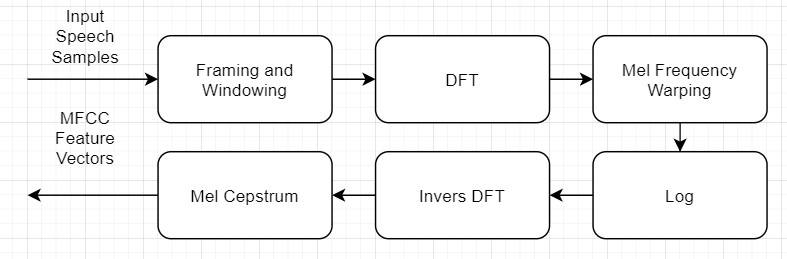
\includegraphics[width=4cm]{figures/1174066/6/1.jpg}
\caption{Teori 1}
\end{figure}

\subsubsection{Konsep dasar neural network}
\hfill\break
Konsep sederhana dari neural network atau jaringan saraf sederhana dengan proses pembelajaran pada anak-anak dengan memetakan pola-pola baru yang diperoleh dari input untuk membuat pola-pola baru pada output. Contoh sederhana ini menganalogikan kinerja otak manusia. Jaringan saraf itu sendiri terdiri dari unit pemrosesan yang disebut neuron yang berisi fungsi adder dan aktivasi. Fungsi aktivasi itu sendiri untuk publikasi diberikan oleh neuron. Jaringan saraf yang mendukung pemikiran sistem atau aplikasi yang melibatkan otak manusia, baik untuk mendukung berbagai elemen sinyal yang diterima, memeriksa kesalahan, dan juga memproses secara paralel. Karakteristik neural network atau jaringan saraf dilihat dari pola hubungan antar neuron, metode penentuan bobot setiap koneksi, dan fungsi aktivasi mereka.
\begin{figure}[H]
\centering
	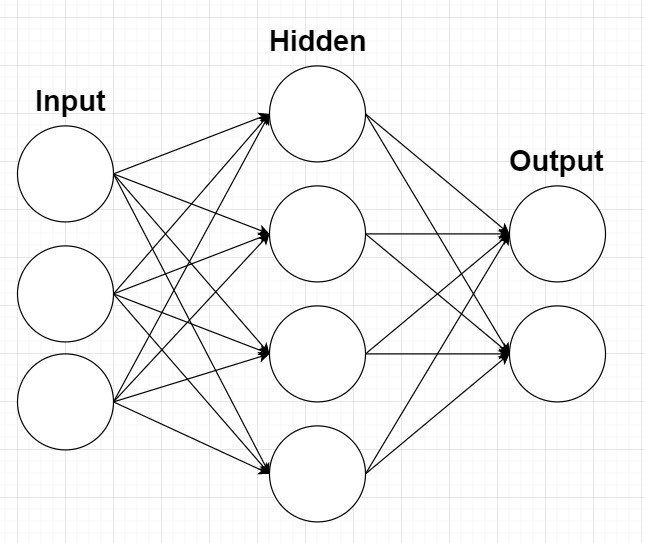
\includegraphics[width=4cm]{figures/1174066/6/2.jpg}
\caption{Teori 2}
\end{figure}

\subsubsection{Konsep pembobotan dalam neural network}
\hfill\break
Pembobotan di dalam neural network juga akan menentukan penanda konektivitas. Dalam proses neural network mulai dari input yang diterima oleh neuron bersama dengan nilai bobot masing-masing input. Setelah memasuki neuron, nilai input akan ditambahkan oleh fungsi penerima. Hasil penambahan ini akan diproses oleh masing-masing fungsi neuron, hasil penambahan ini akan dibandingkan dengan nilai ambang tertentu. Jika nilai jumlah ini melebihi nilai ambang batas, aktivasi neuron akan dibatalkan, tetapi sebaliknya jika jumlah hasil di bawah nilai ambang batas, neuron akan diaktifkan. Setelah neuron aktif maka akan mengirimkan nilai output melalui bobot outputnya ke semua neuron yang terkait.
\begin{figure}[H]
\centering
	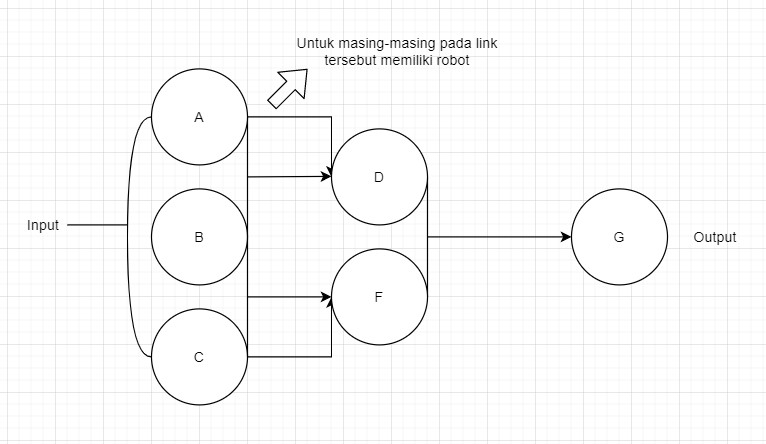
\includegraphics[width=4cm]{figures/1174066/6/3.jpg}
\caption{Teori 3}
\end{figure}

\subsubsection{Konsep fungsi aktifasi dalam neural network}
\hfill\break
Fungsi aktivasi dalam neural network ialah merupakan suatu operasi matematik yang dikenakan pada sinyal output. Fungsi ini digunakan untuk mengaktifkan atau menonaktifkan neuron. Fungsi aktivasi ini terbagi setidaknya menjadi 6, adapun sebagai berikut:
	\begin{enumerate}
	\item Fungsi Undak Biner Hard Limit, fungsi ini biasanya digunakan oleh jaringan lapiran tunggal untuk mengkonversi nilai input dari suatu variabel yang bernilai kontinu ke suatu nilai output biner 0 atau 1.
	\item Fungsi Undak Biner Threshold, fungsi ini menggunakan nilai ambang sebagai batasnya.
	\item Fungsi Bipolar Symetric Hard Limit, fungsi ini memiliki output bernilai 1, 0 atau -1.
	\item Fungsi Bipolar dengan Threshold, fungsi ini mempunyai output yang bernilai 1, 0 atau -1 untuk batas nilai ambang tertentu.
	\item Fungsi Linear atau Identitas.	
	\end{enumerate}
\begin{figure}[H]
\centering
	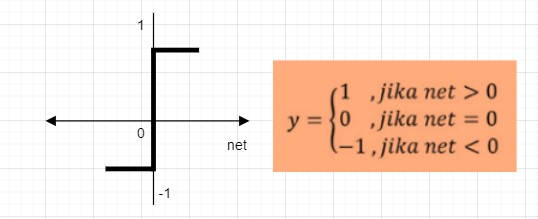
\includegraphics[width=4cm]{figures/1174066/6/4.jpg}
\caption{Teori 4}
\end{figure}

\subsubsection{Cara membaca hasil plot dari MFCC}
\hfill\break
Perhatikan gambar dibawah: Gambar menjelaskan bahwa pada waktu ke-5 kekuatan atau layak yang dikeluarkan pada nada ini paling keras pada 20 Hz, selain itu pada 40 -120 Hz daya atau nilai dikeluarkan pada musik yang telah diplot. Demikian juga, warna terseksi adalah kekuatan atau nilai tertinggi dibandingkan dengan warna canggih. Yang merah terdengar di bawah pendengaran manusia, sehingga tidak bisa didengar secara langsung.
\begin{figure}[H]
\centering
	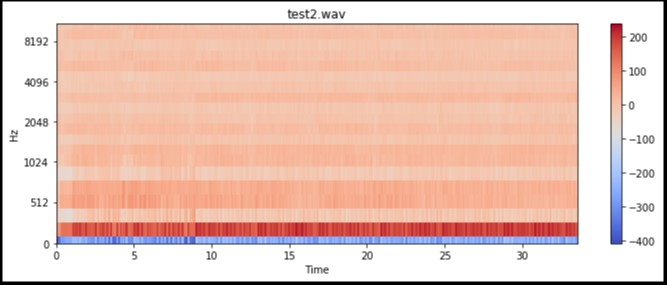
\includegraphics[width=4cm]{figures/1174066/6/5.jpg}
\caption{Teori 5}
\end{figure}

\subsubsection{one-hot encoding}
\hfill\break
one-hot encoding ini adalah untuk mengubah hasil data vektorisasi menjadi angka biner 0 dan 1 dan membuat informasi tentang atribut yang diberi label.
\begin{figure}[H]
\centering
	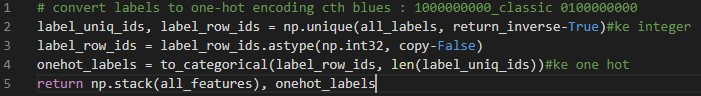
\includegraphics[width=4cm]{figures/1174066/6/6-1.jpg}
\caption{Teori 6-1}
\end{figure}
\begin{figure}[H]
\centering
	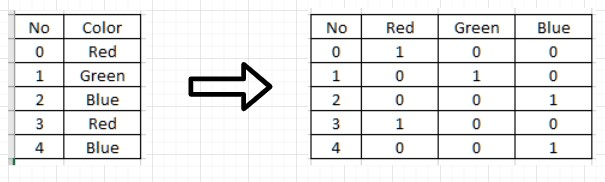
\includegraphics[width=4cm]{figures/1174066/6/6-2.jpg}
\caption{Teori 6-2}
\end{figure}

\subsubsection{Apa fungsi dari np.unique dan to categorical dalam kode program}
\hfill\break
Fungsi np.unique adalah untuk menemukan berbagai elemen atau array unik, dan dapat mengembalikan elemen unik dari array yang diurutkan. Sebagai ilustrasi, cukup bisa dilihat pada gambar di bawah ini. Gambar tersebut menjelaskan bahwa unik itu sendiri akan mengambil data yang berbeda dari variabel a dalam fungsi array.
\begin{figure}[H]
\centering
	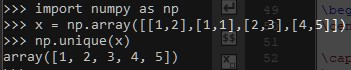
\includegraphics[width=4cm]{figures/1174066/6/7.jpg}
\caption{Teori 7-1}
\end{figure}
Fungsi dari to\_categorical ialah untuk mengubah suatu vektor yang berupa integer menjadi matrix dengan kelas biner. Untuk ilustrasinya bisa dilihat pada gambar \ref{cc71}
\begin{figure}[H]
\centering
	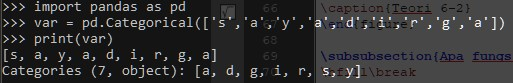
\includegraphics[width=4cm]{figures/1174066/6/7-2.jpg}
\caption{Teori 7-2}
\end{figure}

\subsubsection{Apa fungsi dari Sequential dalam kode program}
\hfill\break
Fungsi dari Sequential sebagai salah satu jenis model yang digunakan dalam perhitungan. Sequential ini membangun tumpukan linear yang berurutan.
\begin{figure}[H]
\centering
	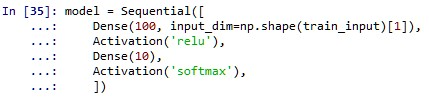
\includegraphics[width=4cm]{figures/1174066/6/8.jpg}
\caption{Teori 8}
\end{figure}


\subsection{Praktek}
\subsubsection{Nomor 1}
\hfill\break
\lstinputlisting[firstline=9, lastline=28]{src/1174066/6/2.py}
Kode di atas menjelaskan isi data GTZAN. Ini adalah kumpulan data yang berisi 10 genre lagu dengan masing-masing genre memiliki 100 lagu yang akan kami lakukan proses MFCC dan juga lagu yang saya pilih, jika GTZAN memiliki beberapa genre jika freesound hanya untuk 1 lagu dan disini kita membuat fungsi untuk membaca file audio dan outputnya sebagai plot
\begin{figure}[H]
\centering
	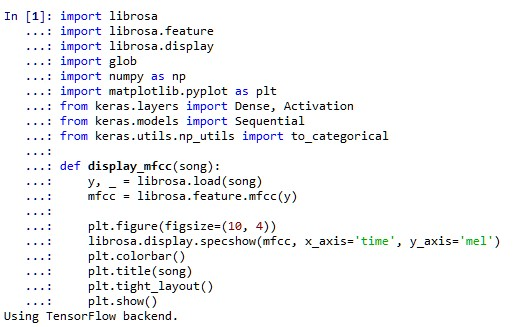
\includegraphics[width=4cm]{figures/1174066/6/no1.jpg}
\caption{Nomor 1}
\end{figure}

\subsubsection{Nomor 2}
\hfill\break
\lstinputlisting[firstline=29, lastline=50]{src/1174066/6/2.py}
Kode di atas akan menampilkan hasil dari proses mfcc yang sudah dibuat fungsi pada soal 1, yaitu display mfcc() dan akan menampilkan plot dari pembacaan file audio. Berikut adalah hasil setelah saya lakukan running dan pembacaan file audio:
\begin{figure}[H]
\centering
	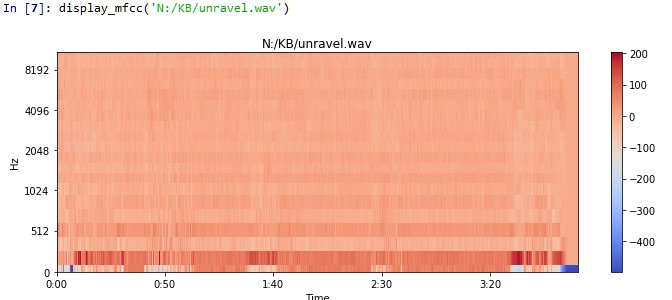
\includegraphics[width=4cm]{figures/1174066/6/no2-1.jpg}
	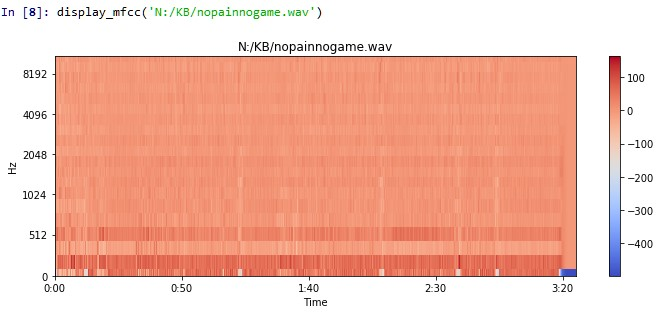
\includegraphics[width=4cm]{figures/1174066/6/no2-2.jpg}
	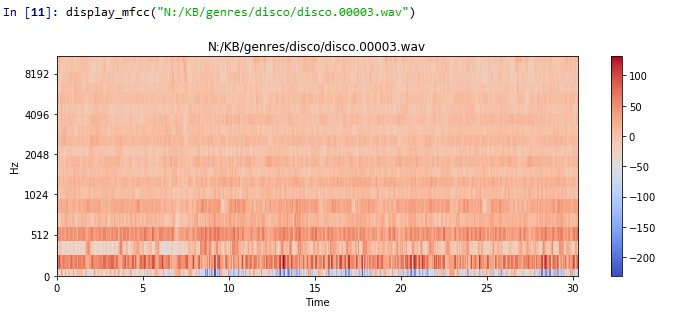
\includegraphics[width=4cm]{figures/1174066/6/no2-3.jpg}
	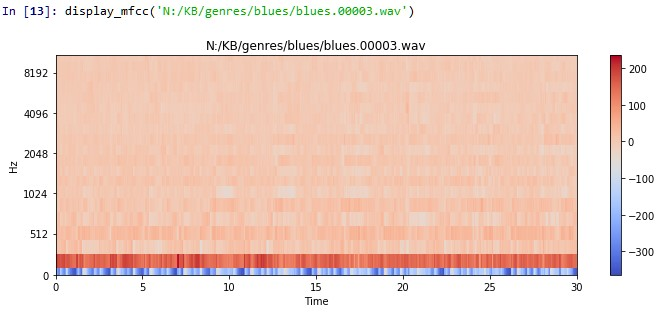
\includegraphics[width=4cm]{figures/1174066/6/no2-4.jpg}
	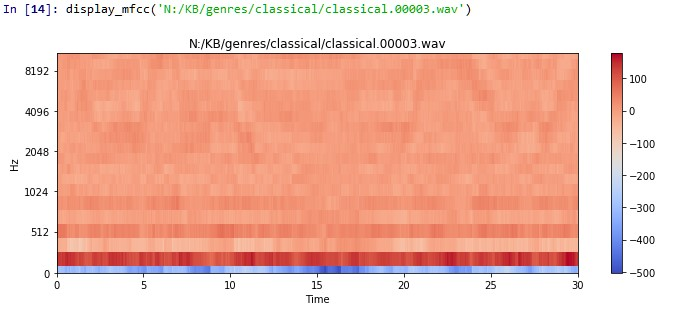
\includegraphics[width=4cm]{figures/1174066/6/no2-5.jpg}
	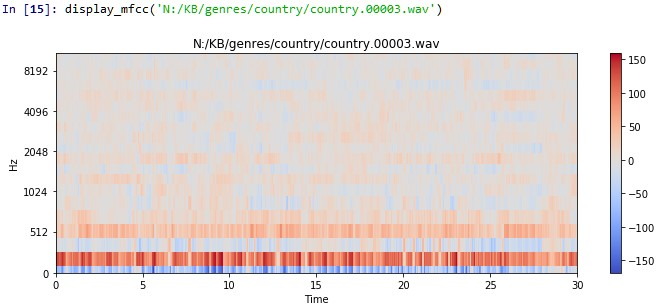
\includegraphics[width=4cm]{figures/1174066/6/no2-6.jpg}
	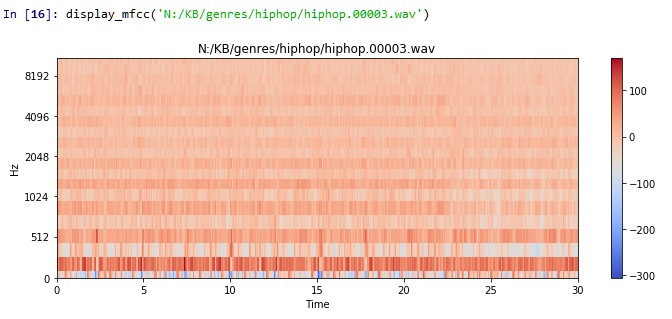
\includegraphics[width=4cm]{figures/1174066/6/no2-7.jpg}
	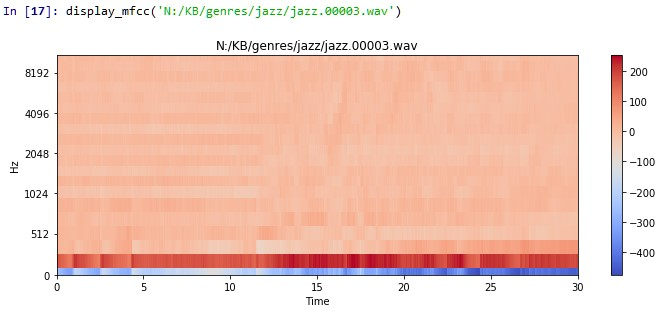
\includegraphics[width=4cm]{figures/1174066/6/no2-8.jpg}
	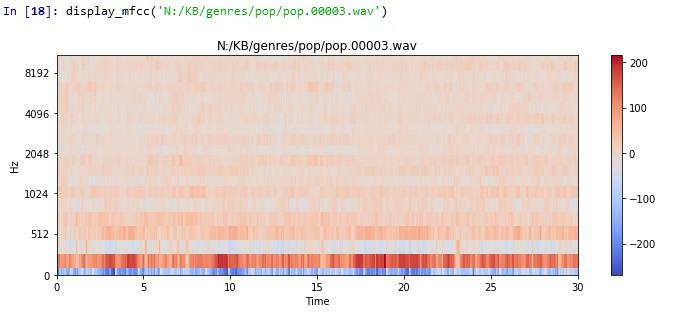
\includegraphics[width=4cm]{figures/1174066/6/no2-9.jpg}
	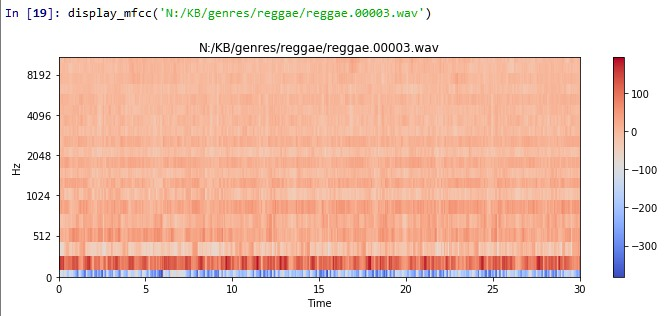
\includegraphics[width=4cm]{figures/1174066/6/no2-10.jpg}
	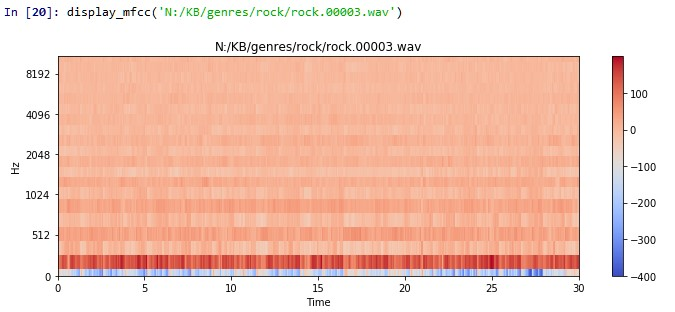
\includegraphics[width=4cm]{figures/1174066/6/no2-11.jpg}
\caption{Nomor 2}
\end{figure}

\subsubsection{Nomor 3}
\hfill\break
\lstinputlisting[firstline=53, lastline=61]{src/1174066/6/2.py}
Baris pertama itu untuk membuat fungsi extract\_features\_song(f). Pada baris kedua itu akan me-load data inputan dengan menggunakan librosa. Lalu selanjutnya untuk membuat sebuah fitur untuk mfcc dari y atau parameter inputan. Lalu akan me-return menjadi array dan akan mengambil 25000 data saja dari hasil vektorisasi dalam 1 lagu.
\begin{figure}[H]
\centering
	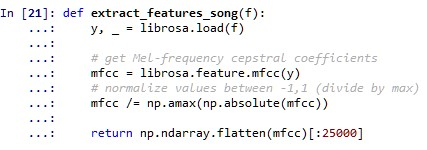
\includegraphics[width=4cm]{figures/1174066/6/no3.jpg}
\caption{Nomor 3}
\end{figure}

\subsubsection{Nomor 4}
\hfill\break
\lstinputlisting[firstline=65, lastline=82]{src/1174066/6/2.py}
Kode di atas dapat digunakan untuk melakukan fungsi yang sebelumnya telah kita lakukan. Kemudian di bagian genre yang disesuaikan dengan dataset nama folder. Untuk baris berikutnya akan mengulang genre folder dengan ekstensi .au. Maka itu akan memanggil fungsi ekstrak lagu. Setiap file dalam folder itu akan diekstraksi menjadi vektor dan akan ditambahkan ke fitur. Dan fungsi yang ditambahkan adalah untuk menumpuk file yang telah di-vektor-kan. Hasil kode tidak menampilkan output.
\begin{figure}[H]
\centering
	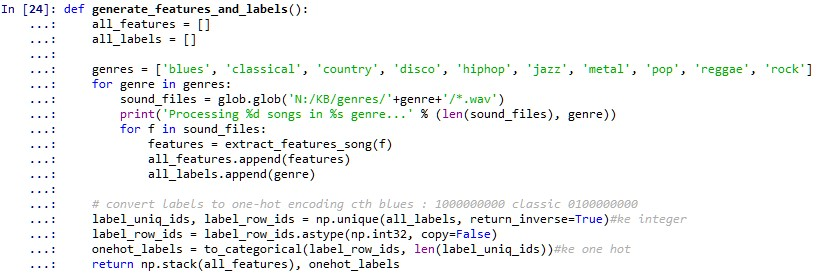
\includegraphics[width=4cm]{figures/1174066/6/no4.jpg}
\caption{Nomor 4}
\end{figure}

\subsubsection{Nomor 5}
\hfill\break
\lstinputlisting[firstline=85, lastline=87]{src/1174066/6/2.py}
Kode diatas berfungsi untuk melakukan load variabel features dan labels. Mengapa memakan waktu yang lama ? Karena mesin akan melakukan vektorisasi terhadap semua file yang berada pada setiap foldernya, di sini terdapat 10 folder dengan masing-masing folder terdiri atas 100 buah lagu, setiap lagu tersebut akan dilakukan vektorisasi atau ekstraksi data menggunakan mfcc. 
\begin{figure}[H]
\centering
	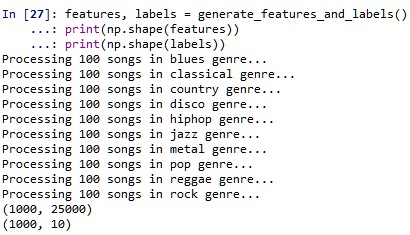
\includegraphics[width=4cm]{figures/1174066/6/no5.jpg}
	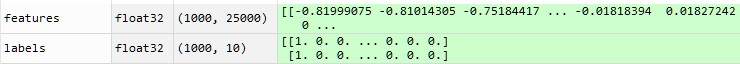
\includegraphics[width=4cm]{figures/1174066/6/no5-1.jpg}
\caption{Nomor 5}
\end{figure}

\subsubsection{Nomor 6}
\hfill\break
\lstinputlisting[firstline=88, lastline=107]{src/1174066/6/2.py}
Kode diatas berfungsi untuk melakukan training split 80\%. Karena supaya mesin dapat terus belajar tentang data baru, jadi ketika prediksi dibuat tentang data yang terlatih itu bisa mendapatkan persentase yang cukup bagus.
\begin{figure}[H]
\centering
	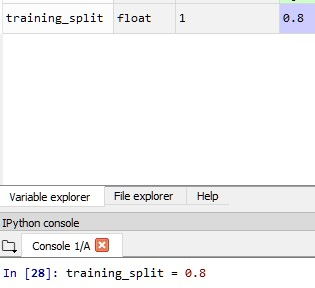
\includegraphics[width=4cm]{figures/1174066/6/no6.jpg}
	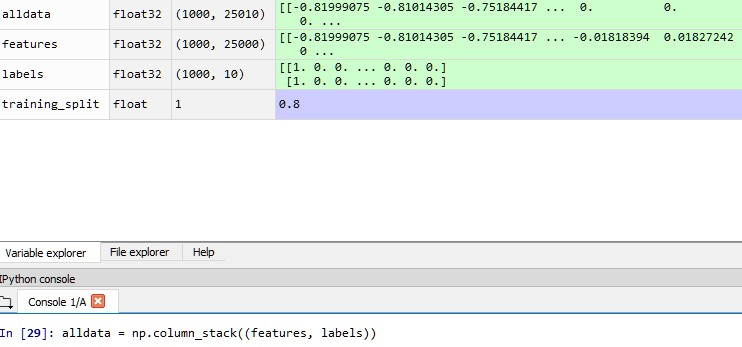
\includegraphics[width=4cm]{figures/1174066/6/no6-2.jpg}
	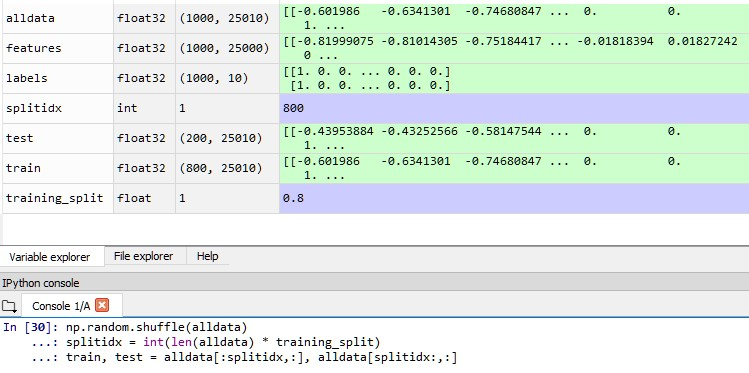
\includegraphics[width=4cm]{figures/1174066/6/no6-3.jpg}
	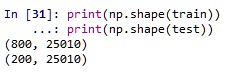
\includegraphics[width=4cm]{figures/1174066/6/no6-4.jpg}
	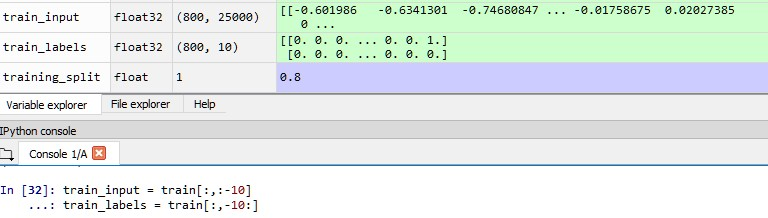
\includegraphics[width=4cm]{figures/1174066/6/no6-5.jpg}
	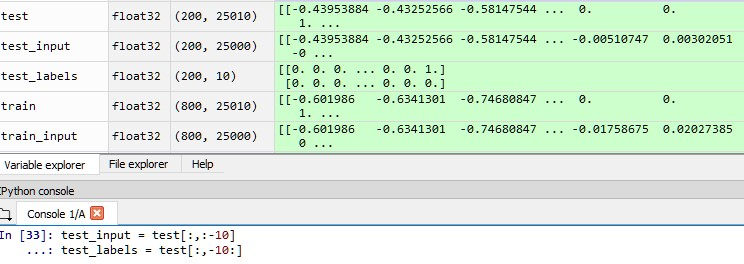
\includegraphics[width=4cm]{figures/1174066/6/no6-6.jpg}
	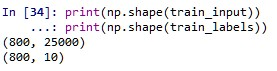
\includegraphics[width=4cm]{figures/1174066/6/no6-7.jpg}
\caption{Nomor 6}
\end{figure}

\subsubsection{Nomor 7}
\hfill\break
\lstinputlisting[firstline=110, lastline=115]{src/1174066/6/2.py}
Fungsi Sequential() ialah Sebuah model untuk menentukan izin pada setiap neuron, di sini adalah 100 dense yang merupakan 100 neuron pertama dari data pelatihan. Fungsi dari relay itu sendiri adalah untuk mengaktifkan neuron atau input yang memiliki nilai maksimum. Sedangkan untuk dense 10 itu adalah output dari hasil neuron yang telah berhasil diaktifkan, untuk dense 10 diaktifkan menggunakan softmax.
\begin{figure}[H]
\centering
	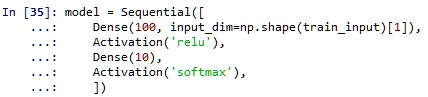
\includegraphics[width=4cm]{figures/1174066/6/no7.jpg}
\caption{Nomor 7}
\end{figure}

\subsubsection{Nomor 8}
\hfill\break
\lstinputlisting[firstline=117, lastline=120]{src/1174066/6/2.py}	
Model Compile di perjelas dengan gambar dibawah, Hasil output pada kode tersebut seperti gambar  menjelaskan bahwa dense pertama itu memiliki 100 neurons dengan parameter sekitar 2 juta lebih dengan aktviasi 100, jadi untuk setiap neurons memiliki masing-masing 1 aktivasi. Sama halnya seperti dense 2 memiliki jumlah neurons sebanyak 10 dengan parameter 1010 dan jumlah aktivasinya 10 untuk setiap neurons tersebut dan total parameternya sekitar 2.5 juta data yang akan dilatih pada mesin tersebut.
\begin{figure}[H]
\centering
	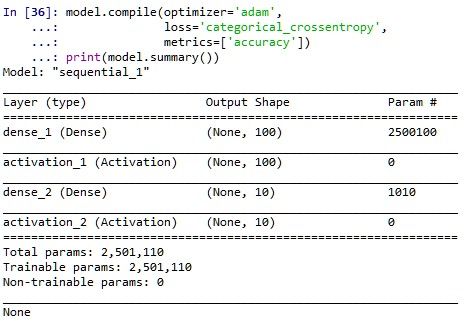
\includegraphics[width=4cm]{figures/1174066/6/no8.jpg}
\caption{Nomor 8}
\end{figure}

\subsubsection{Nomor 9}
\hfill\break
\lstinputlisting[firstline=122, lastline=123]{src/1174066/6/2.py}
Kode tersebut berfungsi untuk melatih mesin dengan data training input dan training label. Epochs ini merupakan iterasi atau pengulangan berapa kali data tersebut akan dilakukan. Batch\_size ini adalah jumlah file yang akan dilakukan pelatihan pada setiap 1 kali pengulangan. Sedangkan validation\_split itu untuk menentukan presentase dari cross validation atau k-fold sebanyak 20\% dari masing-masing data pengulangan.
\begin{figure}[H]
\centering
	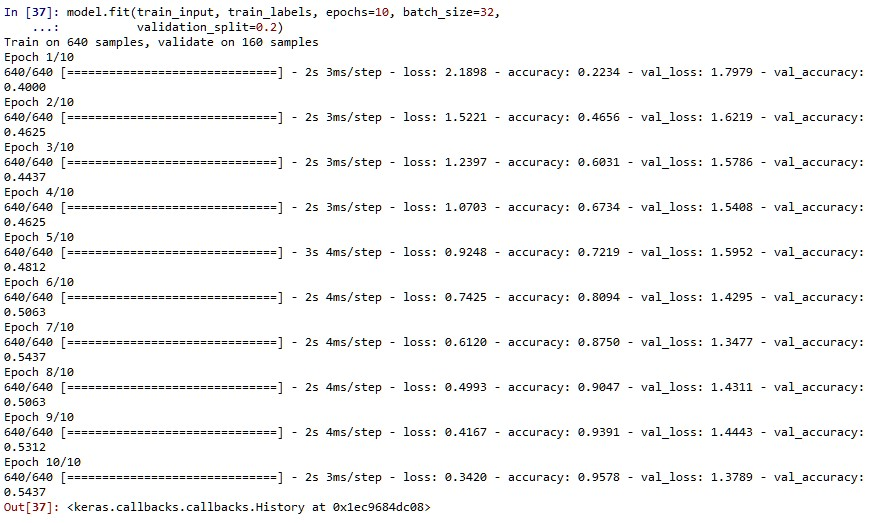
\includegraphics[width=4cm]{figures/1174066/6/no9.jpg}
\caption{Nomor 9}
\end{figure}

\subsubsection{Nomor 10}
\hfill\break
\lstinputlisting[firstline=125, lastline=127]{src/1174066/6/2.py}
Fungsi evaluate atau evaluasi ini ialah untuk menguji data pengujian setiap file. Di sini ada prediksi yang hilang, artinya mesin memprediksi data, sedangkan untuk keseluruhan perjanjian sekitar 55\%.
\begin{figure}[H]
\centering
	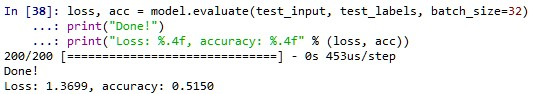
\includegraphics[width=4cm]{figures/1174066/6/no10.jpg}
\caption{Nomor 10}
\end{figure}	

\subsubsection{Nomor 11}
\hfill\break
\lstinputlisting[firstline=130, lastline=130]{src/1174066/6/2.py}
Fungsi Predict ialah untuk menghasilkan suatu nilai yang sudah di prediksi dari data training sebelumnya. Gambar dibawah ini menjelaskan file yang di jalankan tersebut termasuk ke dalam genre apa, hasilnya bisa dilihat pada gambar tersebut presentase yang paling besar yakni genre rock. Maka lagu tersebut termasuk ke dalam genre rock dengan perbandingan presentase hasil prediksi.
\begin{figure}[H]
\centering
	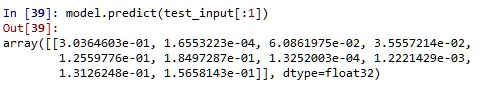
\includegraphics[width=4cm]{figures/1174066/6/no11.jpg}
\caption{Nomor 11}
\end{figure}

\subsection{Penanganan Error}
\subsubsection{Error}
\hfill\break
\begin{itemize}
\item NoBackendError

\begin{figure}[H]
\centering
	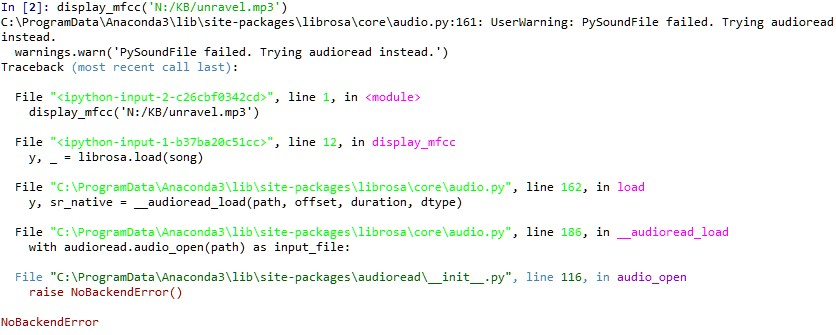
\includegraphics[width=4cm]{figures/1174066/6/error1.jpg}
\caption{NoBackendError}
\end{figure}
\end{itemize}
\subsubsection{Solusi Error}
\hfill\break
\begin{itemize}
\item NoBackendError

Cek kembali file format audionya dipastikan menggunakan wav
\end{itemize}

\subsection{Bukti Tidak Plagiat}
\begin{figure}[H]
	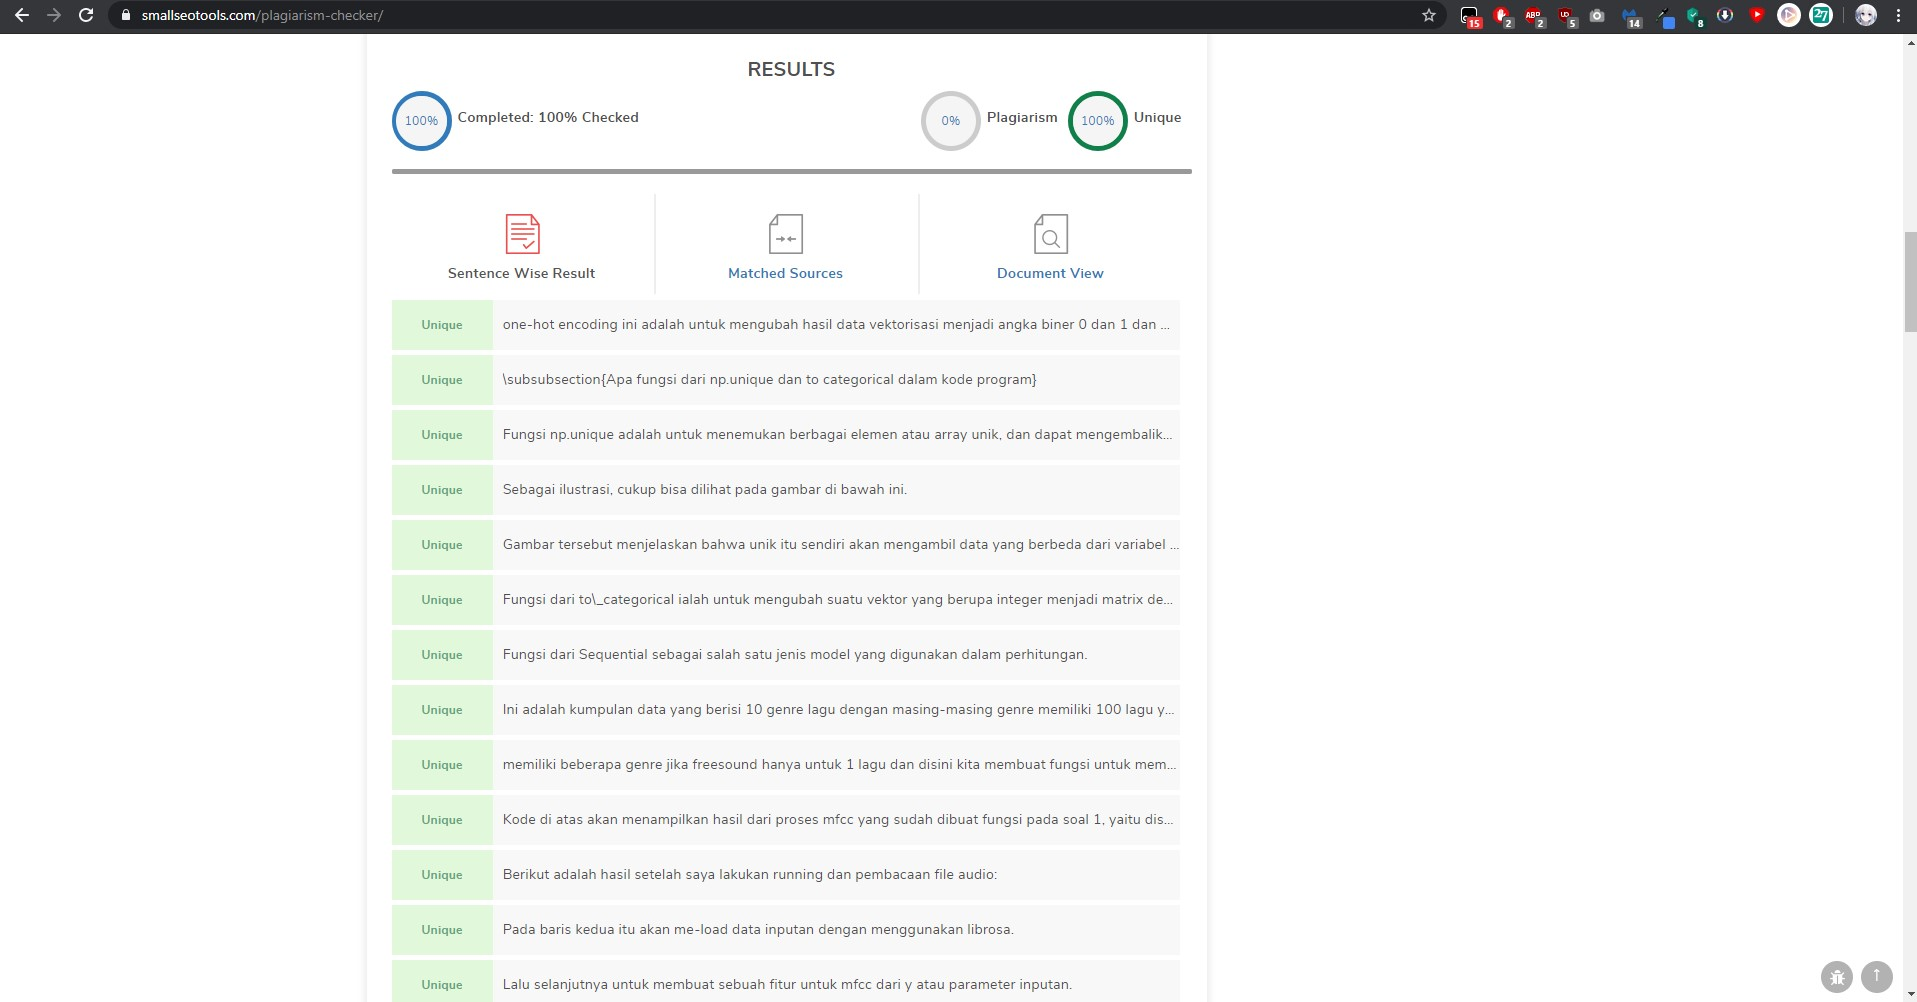
\includegraphics[width=4cm]{figures/1174066/6/buktiplagiat.jpg}
	\centering
	\caption{Bukti tidak plagiat}
\end{figure}

\subsection{Link Youtube}
https://youtu.be/zA7U-zfvI\_w